\documentclass[10pt,xcolor=x11names,compress, show notes]{beamer}% pour l'impression, tout n'apparait qu'une fois \documentclass[handout,12pt]{beamer}

%\usepackage[scaled]{helvet}
\usepackage[round]{natbib}
\usepackage[utf8x]{inputenc}
\usepackage[USenglish]{babel}
\usepackage{todonotes}
\usepackage{color}
\usepackage{pbox}
\usepackage{graphicx}


\usepackage{changepage}
\usepackage{pifont} %pour les symbole sympa \ding{nb}

\usepackage{subfig}

%%% Pour Tikz
\usepackage{tikz}
\usetikzlibrary{calc}
\usetikzlibrary{shapes}
%\usetikzlibrary{arrows,shapes,trees,positioning}  

%%%pour les plots matlab en tikz
\usepackage{pgfplots} 
\pgfplotsset{compat=newest}

%%% Pour les maths
\usepackage{bm}
\usepackage{amsmath,mathtools}
\usefonttheme[onlymath]{serif}
\usepackage{cancel} %pour barrer des math

%%% Pour la mise en forme
\usepackage[export]{adjustbox}
%\usepackage{subcaption}
\usepackage{wrapfig}
\usepackage{pdfpages}
\setbeamertemplate{navigation symbols}{} 
\usepackage{array}
%\usepackage{subfigure}
%\usepackage[]{geometry}
%\usepackage{palatino}
%\setbeamertemplate{caption}{\raggedright\insertcaption\par}
\usepackage{multicol}
\setlength{\columnsep}{0cm}
\usepackage[framemethod=TikZ]{mdframed}


%%% Theme
\def \pied {~~~A.Dinsenmeyer, Q.{Leclère}, J.{Antoni} et E.Julliard~|~\insertshorttitle \hfill \insertframenumber/\inserttotalframenumber~~~} %content if footline
\usetheme{Alice}

%personnalisation
\definecolor{green}{rgb}{0,0.5,0} 

%figure csm
\newlength{\pas}	\setlength{\pas}{0.2cm}
\newcommand{\nbpas}{7}

%\setbeamertemplate{footline}{test}




%\useoutertheme[subsection=false]{miniframes} %%pour avoir le défilement en en-tête des diapos par section
%\setbeamercolor*{lower separation line head}{bg=DeepSkyBlue4} 

% Customisation 
\setlength{\fboxrule}{0.2pt}
\newcommand{\tikzmark}[1]{\tikz[remember picture] \coordinate (#1) ++ (-3pt,6pt) {};}
\newcommand{\citeTransp}[1]{\color{fg!60} \citep{#1}}
\renewcommand\bibsection{\section[]{~}}
\usepackage{algorithm}
\usepackage{algorithmic}
\graphicspath{{images/}}

%% Autre

\definecolor{main}{rgb}{0,0.407843137,0.545098039}%{0 0.439  0.753} %bleu %0 112 192
\definecolor{rouge}{rgb}{1 0.270 0 } %255 69 0
\definecolor{jaune}{rgb}{1 0.745 0} %255 190 0
\definecolor{vert}{rgb}{0.573 0.792 0.209} %146 202 74
\definecolor{source}{rgb}{0,0.5,0} 

\newlength{\avion}
\setlength{\avion}{0.6\textwidth}

\newlength{\larg}	\setlength{\larg}{0.5cm}	
\newlength{\haut}	\setlength{\haut}{4\larg}

\newcommand{\diag}[1]{\lceil#1\rfloor}
\newcommand*\circled[1]{\tikz[baseline=(char.base)]{
            \node[shape=circle,draw,inner sep=2pt,color=main,fill=main!10, line width=1pt] (char) {#1};}}

%%% Page de titre
%======================
\author{\underline{A. {Dinsenmeyer}}$^{1,2}$, Q. {Leclère}$^1$, J. {Antoni}$^1$ et E. Julliard$^3$}
\institute{$^1$ Laboratoire Vibrations Acoustique\\ $^2$ Laboratoire de Mécanique des Fluides et d’Acoustique\\Lyon, France \\ $^3$ Airbus, Toulouse, France}
\title{Comparison of microphone array denoising techniques and application to flight test measurements}
\subtitle{}
\titlegraphic{ \includegraphics[height=1cm]{logo/LABEX_CELYA.jpg} \hfill
 	  \includegraphics[trim={0 3cm 0 3cm},clip=true,height=1cm]{logo/logo_ADAPT.png} \hfill
 \includegraphics[height=1cm]{logo/LVA_compact_couleur.jpg} \hfill
 \includegraphics[height=1cm]{logo/logo_lmfa.pdf} \hfill  }
\date{\small \vfill AIAA/CEAS Aeroacoustics Conference -- May 23, 2019 }
\begin{document}

%%%		Title
%======================
\begin{frame}[plain,t]
	\maketitle	
\end{frame}

%%% Context
%======================
\section*{Context}
\begin{frame}[t]{\insertsectionhead}
\vspace{0.2cm}
\begin{overlayarea}{\textwidth}{0.3\textheight}
\only<1-2>{
	\noindent\begin{minipage}{1.1\textwidth}
		\begin{itemize}
		        \item<1-> \textbf{Unwanted noise} : electronic, ambient, flow-induced, \dots
		        	\item<1-> \textbf{Multi-channel acquisition} : inflight/wind tunnel tests for aircraft design\\			
		        \item<2-> 2 kinds of pressure excitation: \\
			$ \left. \begin{array}{l} 
			\mbox{- from the acoustic sources (\textcolor{source}{signal})} \\                   
			\mbox{- from the turbulent boundary layer (\textcolor{rouge}{noise})}                      
			\end{array} \right\} \mbox{~very low SNR}$ 
		\end{itemize}
\end{minipage}
}
\end{overlayarea}
\vfill
\begin{minipage}{\textwidth}
		\centering
		\includegraphics<1>[width=\avion]{avion2.eps}
		%\includegraphics<2>[width=\avion]{avion2.eps}
		%\includegraphics<+>[width=\avion]{avion3.eps}
		%\includegraphics<3>[width=\avion]{avion4.eps}
		\includegraphics<2->[width=\avion]{avion5.eps}
	\end{minipage}
	
\end{frame}

\begin{frame}[t]{\insertsectionhead}
	\begin{center}
		\textcolor{black}{\bfseries \centering  How to separate the acoustic sources from the noise ?}
	\end{center}
	\vfill
{ \bfseries Existing methods:}
\small
	\begin{itemize}
        		\item physical removal : windscreen, mic recession, porous treatment,\dots
        		\item background subtraction $\rightarrow$ not always available or representative
        		\item wavenumber filtering $\rightarrow$ requires high spatial sampling
        		\item diagonal removal $\rightarrow$ underestimation of source level
        		\item other post-processing (inverse problem) $\rightarrow$ for long records
	\end{itemize}

	\vfill
\onslide<2->{
{\bfseries We propose a new method}
\small
	\begin{itemize}
		\item Solve an inverse problem to recover the source signal
	\end{itemize}
	\vfill
{\bfseries and compare it } to an existing method
\small
\begin{itemize}
        \item Use noise-free channels as references
\end{itemize}

}
\end{frame}

\begin{frame}{Outline}
	\tableofcontents[]
\end{frame}

\section{CSM properties}

%\begin{frame}{\insertsectionhead}
%	\centering
%	\small Spectres moyennés (processus stationnaire)\\[1em]
%	\begin{tikzpicture}	
%		\node (mic) at (0,0) {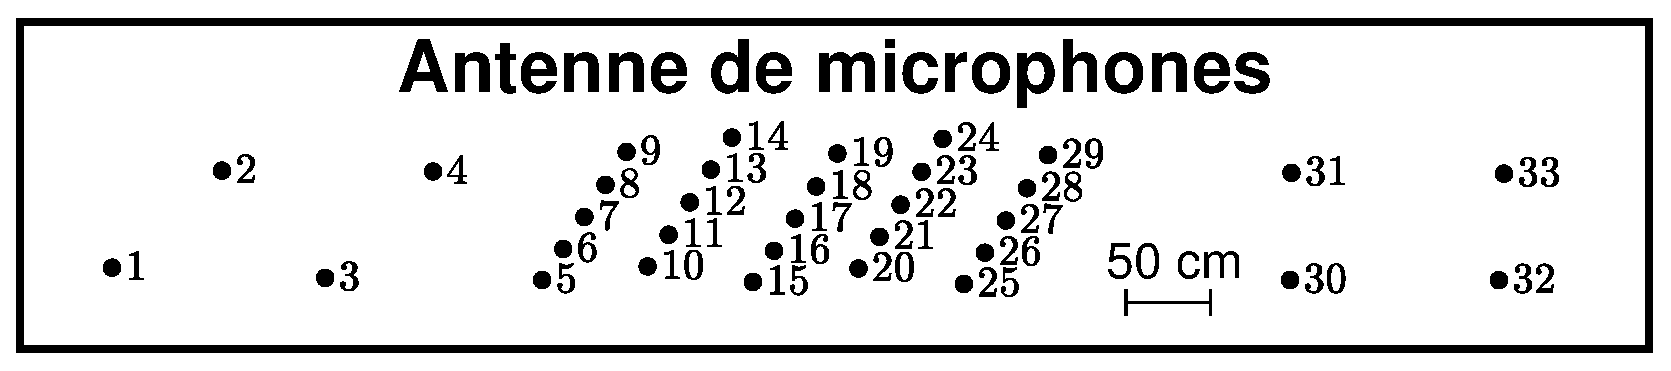
\includegraphics[width=4cm]{mic.eps}};
%		\node[align=center,font=\scriptsize] (mic2) at ($(mic.east)+(2cm,0)$) { ${p}_1(f)$ \\$\dots$\\ ${p}_M(f)$};
%		\draw[->,>=stealth] (mic.east) to ($(mic2.north west)-(0,1.8ex)$);
%		\draw[->,>=stealth,dotted] (mic.east) to (mic2.west);
%		\draw[->,>=stealth] (mic.east) to ($(mic2.south west)+(0,1.8ex)$);
%	\end{tikzpicture}
%	\vspace{1cm}
%	\vfill
%	\begin{tikzpicture}		
%		\uncover<5->{
%		\draw[->,>=stealth] (0,\nbpas\pas) to ++($(-\nbpas\pas,\nbpas\pas/2)+(-2\pas,\pas)$) ;
%		\node at ($(0,\nbpas\pas)+((-\nbpas\pas,\nbpas\pas/2)+(0,0.5em)$) {...};
%		\node at ($(0,\nbpas\pas)+((-\nbpas\pas,\nbpas\pas/2)-(0.5em,0.5em)$) {\footnotesize $f$};
%		\begin{scope}[transparency group,opacity=0.5]
%			\draw[step=\pas,draw=black,fill=gray!30,thin,xshift=-\nbpas\pas,yshift=\nbpas\pas/2]  (0,0) grid (\nbpas\pas,\nbpas\pas) rectangle (0,0);
%			\draw[step=\pas,draw=black,fill=gray!30,thin,xshift=-\nbpas\pas/2,yshift=\nbpas\pas/4]  (0,0) grid (\nbpas\pas,\nbpas\pas) rectangle (0,0);
%		\end{scope}
%		}
%		\uncover<2->{
%		\node at ($(0,\nbpas\pas)+(3.5\pas,3\pas)$) {\small $\bm{S}_{pp}(f)$};
%		\draw [fill=gray!30] (0,0) rectangle ++(\nbpas\pas,\nbpas\pas) ;
%		\draw[step=\pas,black,thin] (0,0) grid (\nbpas\pas,\nbpas\pas);
%		\foreach \xtick in {1,...,\nbpas} { \node at (\xtick\pas-0.5\pas,\nbpas\pas+1ex) {\scriptsize\pgfmathprintnumber{\xtick}}; }
%		\foreach \ytick [count=\ny from 1] in  {\nbpas,...,1} { \node at (-1ex,\ytick\pas-0.5\pas) {\scriptsize\pgfmathprintnumber{\ny}}; }
%		\foreach \x in {1,...,\nbpas}{			
%			\draw [fill=white] (\x\pas-\pas,\nbpas\pas-\x\pas) rectangle ++(\pas,\pas) ;			
%		}
%		}
%		\uncover<3->{
%			\draw [fill=black!70] (0\pas,1\pas) rectangle ++(\pas,\pas) ;
%			\node (inter) at (0+0.5\pas, \pas+0.5\pas) {};
%			\node[anchor=north west,align=center,font=\footnotesize] (inter2) at ($(inter)+(0.5cm,-0.5cm)$)  {   Corrélation entre \\  les micros 1 et 6\\ $\Rightarrow$  \bfseries interspectre};
%			\draw[->,>=stealth] (inter) to [out=-90,in=160] ($(inter2.north west)-(0,1ex)$) ;
%		}
%		\uncover<4->{
%			\draw [fill=black!70] (2\pas,4\pas) rectangle ++(\pas,\pas) ;
%			\node (auto) at (2\pas+0.5\pas, 4\pas+0.5\pas) {};
%			\node[anchor=north west,align=center,font=\footnotesize] (auto2) at (\nbpas\pas,\nbpas\pas+0.7cm)  {  \bfseries autospectre};
%			\draw[->,>=stealth] (auto) to [out=90,in=200] ($(auto2.south west)+(0,1ex)$) ;
%		}
%			
%	\end{tikzpicture}  
%	\vfill 
%\end{frame}

%%% CSM properties
%======================
\begin{frame}[t]{\insertsectionhead}
\centering
	
	 \hfill \includegraphics[width=3cm,valign=m]{idee.png}  \hfill \onslide<2->{\small $\bm{S}_{xy} =\frac{1}{I}\sum_{i=1}^{I}\bm{x}_i\bm{y}_i^H$} 

	\vfill

\begin{overlayarea}{\textwidth}{0.4\textheight}
	\alt<1-1>{\small At one frequency and for $i=1,\dots,I$ snapshots}{\small At one frequency, for averaged Cross-Spectral Matrix:} \onslide<3->{$I\rightarrow \infty$}
	\only<1>{
	$$\underbracket[0.5pt]{~\bm{p}_i~}_{\text{measured spectra}} =\underbracket[0.5pt]{~\textcolor{source}{\bm{a}}_i~}_{\text{acoustic part}} + \underbracket[0.5pt]{~\textcolor{rouge}{\bm{n}}_i~}_{\text{unwanted noise}} $$
	}
	\only<3->{$$\underbracket[0.5pt]{~\bm{S}_{pp}~}_{\text{measured CSM}} =\underbracket[0.5pt]{ ~\textcolor{source}{\bm{S}_{aa}}~}_{\text{acoustic CSM}} +\underbracket[0.5pt]{\bcancel{~\textcolor{rouge}{\bm{S}_{nn}}~}}_{\parbox[t]{2.2cm}{\centering \text{\scriptsize unwanted noise} \\ $\approx$ \scriptsize diagonal matrix }} + \underbracket[0.5pt]{\bcancel{~\bm{S}_{an}+\bm{S}_{na}}}_{\parbox[t]{2cm}{\centering  \text{\scriptsize cross-terms}\\ $\rightarrow 0$ }}$$
	}	
	\only<2>{$$\underbracket[0.5pt]{~\bm{S}_{pp}~}_{\text{measured CSM}} =\underbracket[0.5pt]{ ~\textcolor{source}{\bm{S}_{aa}}~}_{\text{acoustic CSM}} +\underbracket[0.5pt]{~\textcolor{rouge}{\bm{S}_{nn}}~}_{\parbox[t]{2cm}{\centering \text{\scriptsize unwanted noise} \\ ~}}  + \underbracket[0.5pt]{~\bm{S}_{an}+\bm{S}_{na}}_{\parbox[t]{2cm}{\centering  \text{\scriptsize cross-terms}\\ ~ }}$$
	}
	
	
	
	\onslide<3->{
	\centering
	\setlength{\larg}{0.3cm}	
	 \setlength{\haut}{1.3cm}
	 \setlength{\tabcolsep}{0.7ex}
	 \hspace{-1.5cm}\tikz{
		 	\node at (0,0) (a) {};
		 	\draw [rectangle,main,line width=1pt,fill=main!10] (a)  rectangle  ++ (\larg,-\haut)  ; 	 
		 	%\draw[rectangle,main,line width=1pt,fill=main!10] (a)++(\larg+0.1cm,-0.5\haut+0.5\larg) rectangle ++(\larg,-\larg);
			\draw[main,rectangle,line width=1pt,fill=main!10] (a)++(1\larg+0.1cm,-0.5\haut+0.5\larg) rectangle ++(\haut,-\larg);
			\node at ($(a)+(2.5\larg+\haut,-0.5\haut)$) {$+$};
			\node at ($(a)+(-\larg,-0.5\haut)$) {$=$};
		} 
		\tikz{
			\draw[main,line width=1pt]  (-0.9cm,0) rectangle ++(\haut,-\haut); 
			\draw[line width=1pt,main] (-0.9cm,0) to ++(\haut,-\haut);
		}	
		}
\end{overlayarea}	

	\begin{itemize}
		\setlength{\itemindent}{1cm}
		\item<3-> \textcolor{rouge}{TBL noise} with \textbf{short} spatial correlation: {\bfseries diagonal CSM}\\		
		\item<3-> \textcolor{source}{Acoustic field} - with \textbf{high} spatial correlation \\
		\hspace{3cm} - few equivalent monopoles: {\bfseries low-rank CSM}\\ %\centering few uncorrelated monopoles
	\end{itemize}
\end{frame}


\section{Probabilistic Factor Analysis (PFA)}
\begin{frame}
\tableofcontents[currentsection,hideothersubsections]
\end{frame}
\subsection*{Statistical model}
\begin{frame}{\insertsectionhead}
	\vfill
	\begin{itemize}
        		\item<1-> \textbf{Statistical model}\\
        		\small At one frequency and for the i$^{th}$ snapshot:\\    ~\\    	
        		\hspace{-6em}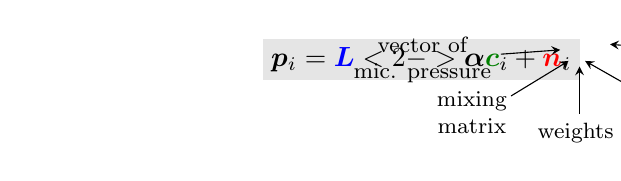
\begin{tikzpicture}[remember picture]
			\colorbox{gray!20}{$\tikzmark{p}\bm{p}_i = \tikzmark{L}\textcolor{blue}{\bm{L}}
			\uncover<2->{\tikzmark{alpha}\bm{\alpha}}
			 \tikzmark{c}\textcolor{green}{\bm{c}}_i + \tikzmark{n}\textcolor{red}{\bm{n}}_i$}
			
			%p
			\node (pdescr) [below left=-0.5cm and 1cm of p, align=center,font=\footnotesize]{
				vector of\\mic. pressure
			};
			\draw[->,>=stealth] (pdescr) -- ($(p.east)+(-7pt,6pt)$);
			
			% L
			\node(Ldescr) [below left=0.2cm and 0.8cm of L,align=center,font=\footnotesize] {
				 mixing \\matrix
			};
	    		%\draw[] (Ldescr.east) to [in=-90,out=45]  (L.south) ;
	    		\draw[->,>=stealth] ($(Ldescr.east)+(-2pt,6pt)$) to ($(L)+(-4pt,2pt)$);
	    		
	    		%alpha
	    		\uncover<2->{
	    		\node (adescr) [below=0.6cm of alpha,font=\footnotesize,align=center]{
	    		weights
	    		};
	    		\draw[->,>=stealth] (adescr) to ($(alpha.south)$);
	    		}
	    		
	    		% c
	    		\node(cdescr) [below right  =0.3cm  and 0.8cm of c , align=center,font=\footnotesize]{
	    			vector of\\latents factors
	    		};
	    		\draw[->,>=stealth] ($(cdescr.north west)+(3pt,-3pt)$) to ($(c.south)+(2pt,2pt)$);
	    		
	    		% n
	    		\node(ndescr) [below right=-0.5cm and 1cm of n,align=left,font=\footnotesize]{
	    			noise (+model errors)
	    		};
	    		\draw[->,>=stealth] (ndescr.west) to ($(n.east)+(11pt,8pt)$);
		\end{tikzpicture}
		
		\begin{itemize}
		        \item Capture dominant correlation with few factors (close to PCA) \\
		        $\hookrightarrow$ low-rank acoustic CSM : $\bm{S}_{aa}=\textcolor{blue}{\bm{L}}\textcolor{green}{\bm{S}_{cc}}\textcolor{blue}{\bm{L}}^H$
		        \item Extract anisotropic noise\pause
		        \item Weights enforce sparsity $\rightarrow$ lower the number of factors\\
		        \item Strong data compression 
		\end{itemize}
	\end{itemize}
	\vfill
        	\begin{overlayarea}{\textwidth}{0.5\textheight}
        	\onslide<3->{
	\begin{itemize}        		
        		\item \textbf{Bayesian approach : } See parameters as random variables\\[1ex]
        		\renewcommand{\arraystretch}{1.5}    		
        		\hspace{-1cm}\begin{tabular}{|c|c|c|c|}
        		\hline
        		$\textcolor{blue}{\bm{L}}\sim\mathcal{N}_{\mathbb{C}}(0,\diag{\frac{\bm{1}}{K}})$& 
		$\textcolor{green}{\bm{c}}_i\sim\mathcal{N}_{\mathbb{C}}(0,\diag{\bm{\gamma}^2})$&
		$\textcolor{rouge}{\bm{n}}_i\sim\mathcal{N}_{\mathbb{C}}(0,\diag{\bm{\sigma}_n^2})$&
		$\bm{\alpha}\sim\mathcal{E}(a_\alpha)$\\\hline
		\end{tabular}       \\[0.5ex]
		+ hyperparameters : $\bm{\gamma}^2, \bm{\sigma}^2\sim\mathcal{IG}(\bm{a}_{\gamma,\sigma},\bm{b}_{\gamma,\sigma})$\\[1ex]      	
%		\pause			 
%        		   \vfill     		
%        		\item \textbf{Solved using MCMC algorithm} (Gibbs sampling)\\
%		\small Iterative draws in the marginal conditional distributions of each parameter\normalsize
%		\pause		
%        		 \vfill 
%        		 \vspace{-0.5em}
%        		 \item \textbf{Finally}, signal CSM: 
%        		 \hspace{4ex}\parbox{0.3\textwidth}{
%        		 $$\bm{\hat{S}}_{aa}=\frac{1}{N_s}\sum_{i=1}^{N_s}\textcolor{blue}{\bm{L}}\textcolor{green}{\bm{c}}_i\textcolor{green}{\bm{c}}^H_i\textcolor{blue}{\bm{L}}^H$$        
 %       		}
	\end{itemize}
	}		
	\end{overlayarea}	
\end{frame}

\begin{frame}{\insertsectionhead ~-- Optimization}
	\centering
	\begin{tikzpicture}
		\node (pic) {\fbox{\includegraphics[width=0.44\textwidth]{modele.png}}};
		\node (mod) [right=0.7 of pic,align=center] {
			\textbf{Parametric model}: $\mathcal{M}(\bm{\theta})$\\
			\small with $\bm{\theta} = \left\{\bm{L},~\bm{\alpha},~\bm{c},~\bm{n},~\bm{a}_{\gamma,\alpha,\sigma},~\bm{b}_{\gamma,\sigma}\right\}$
		};
		\draw[->,>=stealth,line width=1pt] (pic) to (mod);
	\end{tikzpicture}
	\vfill	
	\begin{tabular}{c c}
		\textbf{Optimization step}:&
		$\boxed{ \displaystyle  \bm{\theta} =\underset{\bm{\theta}}{\arg\!\max} \underbrace{\text{P} \left( \bm{\theta} \mid \bm{S}_{pp}\right)}_{ \text{\pbox{7cm}{\centering \normalsize objective function}}}}$ %fr :  fonction obectif	
	\end{tabular}
	\vfill
	\flushleft
	\begin{itemize}
        		%\item The input data is the averaged CSM
        		\item The objective function is the joint posterior probability\\  $\hookrightarrow$ no closed-form	$\rightarrow$ approximated with numerical methods
\end{itemize}
	
	%The fitness function is the posterior probability $\rightarrow$ has no close form\\
	%$\hookrightarrow$ approximation with numerical methods
	


\end{frame}





\newlength{\wg} \setlength{\wg}{0.4\textwidth}
\begin{frame}{\insertsectionhead~-- Optimization}
\textbf{Maximizing the posterior probability distribution}\\% iterative ; biaised random walk
{\itshape ~~~~$\hookrightarrow$ Find the optimal parameter set that best fits the data}\\
%~~~~$\hookrightarrow$ Numerical method: the Gibbs sampler}%performs an iterative biased random walk
\vfill
\begin{overlayarea}{\textwidth}{0.5\textheight}
	\begin{minipage}{0.59\textwidth}
	\vfill
	\begin{itemize}
		\item Numerical method: the Gibbs sampler
		\item MCMC algorithm
		\item Global optimization process
	       % \item perform a biased random walk through the target distribution
	\end{itemize}
	\end{minipage}
	\hfill
	\begin{minipage}{0.4\textwidth}
	\centering
		\only<1>{\vspace{0.97\wg}}
		\includegraphics<2>[trim=-1.66cm 0 0 0, clip,height=\wg,angle=-90]{model2.pdf}
		\includegraphics<3>[trim=-1.66cm 0 0 0, clip,height=\wg,angle=-90]{model0.pdf}
		\includegraphics<4>[trim=-1.66cm 0 0 0, clip,height=\wg,angle=-90]{model3.pdf}
		\includegraphics<5>[trim=-1.66cm 0 0 0, clip,height=\wg,angle=-90]{model4.pdf}
		%\includegraphics<5>[trim=-1.66cm 0 0 0, clip,height=\wg,angle=-90]{model5.pdf}
		\includegraphics<6>[trim=-1.66cm 0 0 0, clip,height=\wg,angle=-90]{model6.pdf}
		\includegraphics<7>[trim=-1.66cm 0 0 0, clip,height=\wg,angle=-90]{model7.pdf}
		\includegraphics<8->[height=\wg+0.002\textwidth,angle=-90]{model8.pdf}
	\end{minipage}
	
\end{overlayarea}
\vfill
\onslide<9->{	
	\footnotesize Example of inflight measurements\\
	\centering
	\begin{tabular}{c c c c c c c}
	\footnotesize Measured CSM && \footnotesize Signal CSM && \footnotesize Noise CSM && \footnotesize Residual CSM\\
	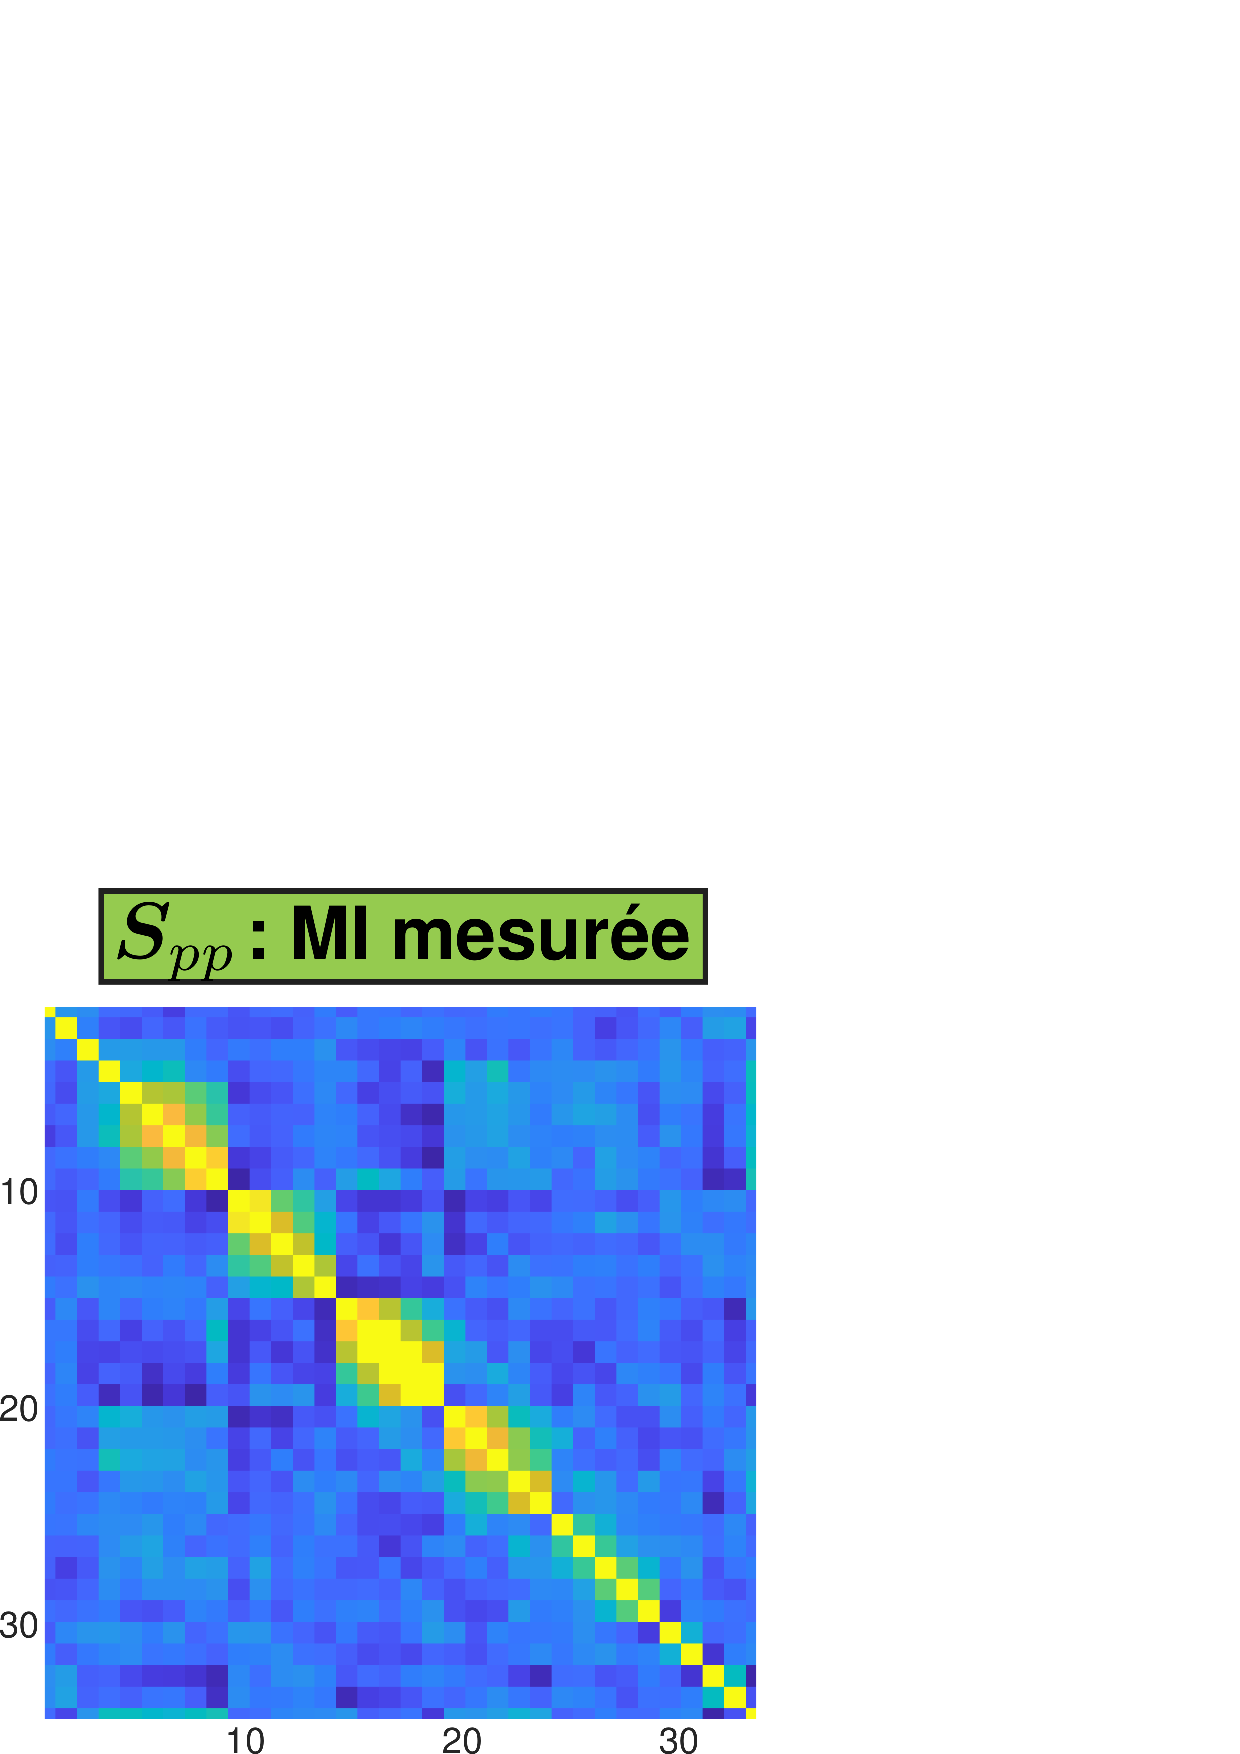
\includegraphics[valign=m,width=0.17\textwidth]{csm.png} &= & \includegraphics[valign=m,width=0.17\textwidth]{signal.png} & +&  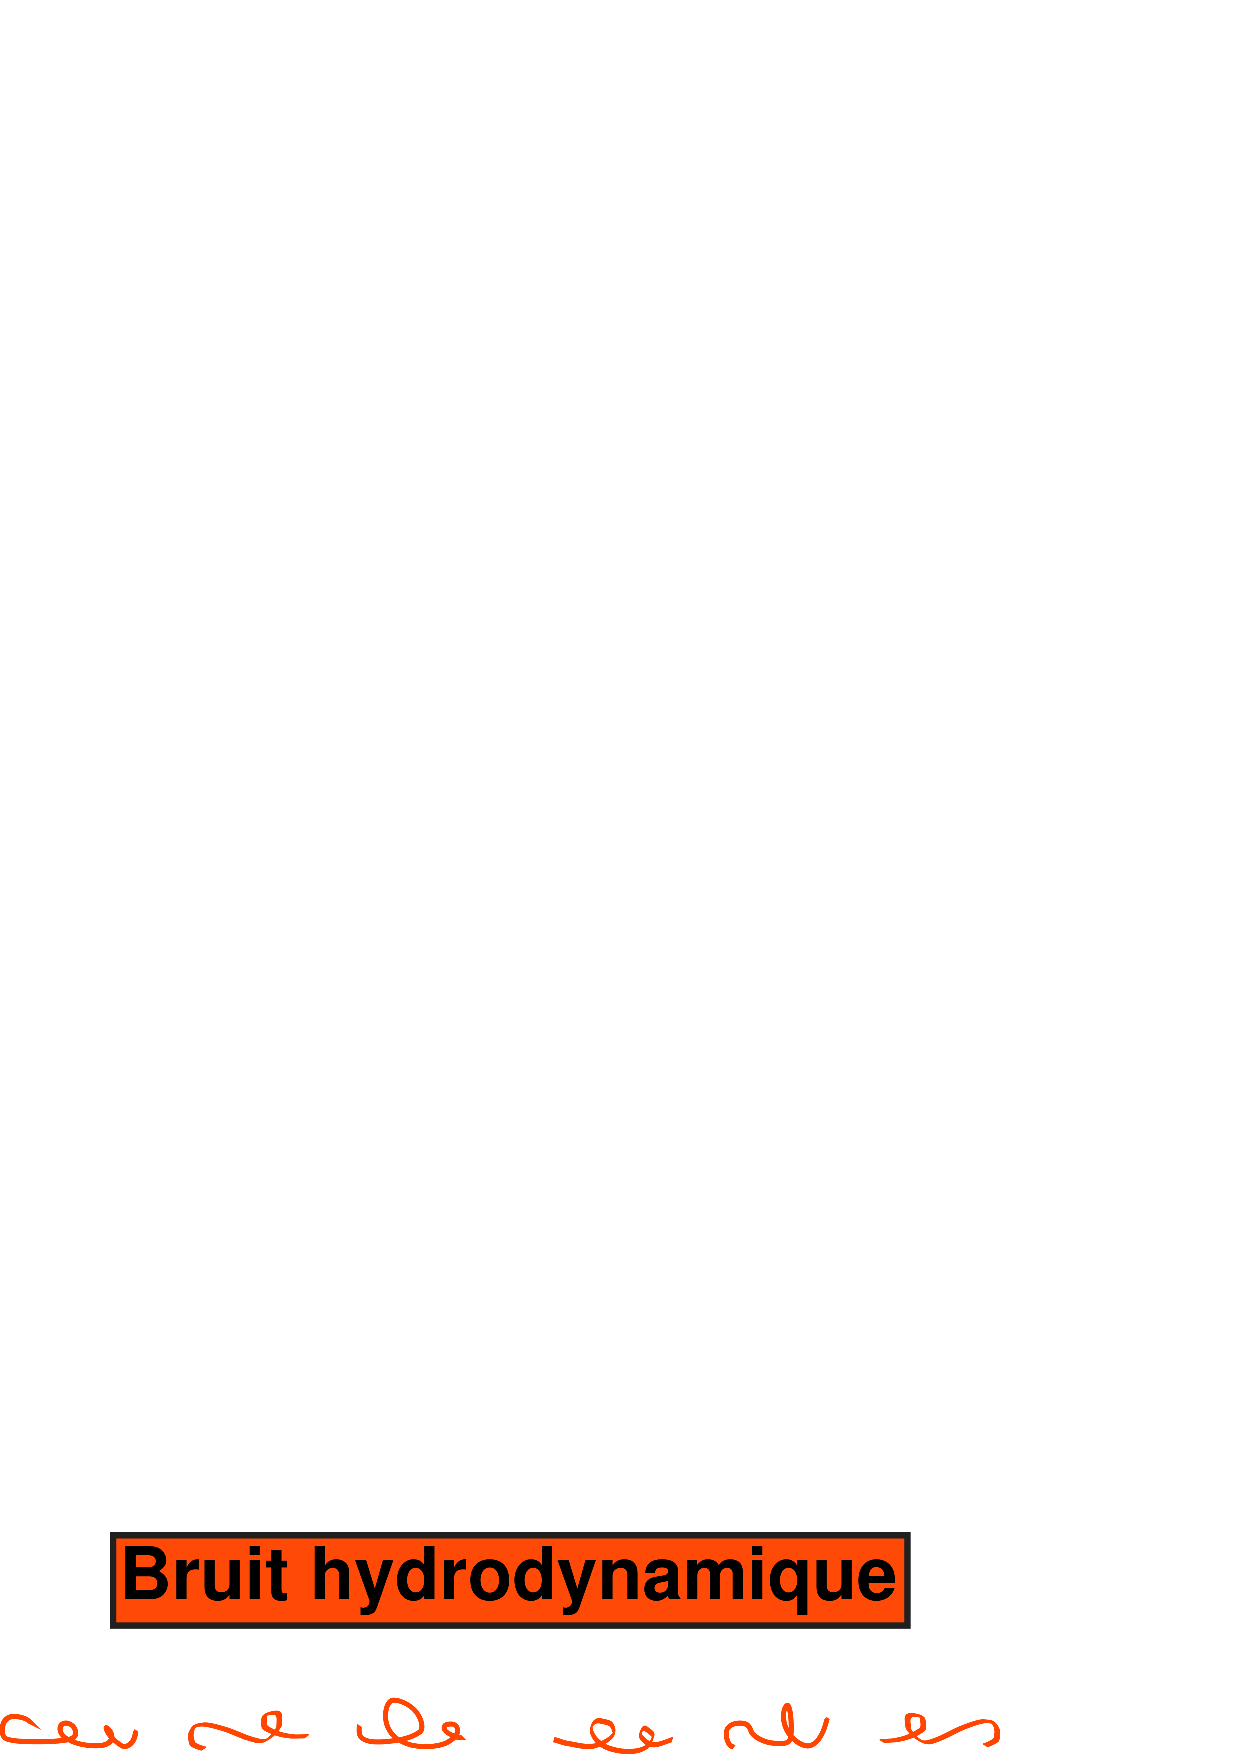
\includegraphics[valign=m,width=0.17\textwidth]{bruit.png} &+&\includegraphics[valign=m,width=0.17\textwidth]{error_csm.png}\\% \pbox{0.2\textwidth}{}\\
	\end{tabular}
	\vfill
}
\end{frame}

\begin{frame}{\insertsectionhead}
\vfill
\onslide<1->{
\hspace{-0.5cm}\begin{minipage}[t]{0.58\textwidth}
~\centerline{\resizebox{0.5cm}{!}{\circled{\textbf{+}}}} \\
\begin{itemize}
        \item[$\bullet$] The bayesian approach:
        \begin{itemize}
   	     \item prior knowledges are part of the model
   	     \item gives credible interval
	\end{itemize}
	~\\
	\item[$\bullet$] Probabilistic Factor Analysis :
	\begin{itemize}
   	     \item preserves the CSM properties
   	     \item reduces data dimension
   	     \item  no input parameter to set
   	     \item blind: no hypothesis on the source
   	     %\item can denoise several measurement datasets
	\end{itemize}
\end{itemize}
\vfill
\end{minipage}
}
\hfill
\pause
\begin{minipage}[t]{0.41\textwidth}
~\centerline{\resizebox{0.5cm}{!}{\circled{\raisebox{-1ex}{\textbf{$\:$-$\:$}}}}}\\[1ex]
\begin{itemize}
        \item[-] \small Sensitive to prior choices\\ esp. for ill-posed problem
        \item[-]  \small Computationally expensive
\end{itemize}
\vfill
\end{minipage}\\
\vfill
\end{frame}


\section{Denoising with reference channels}
\begin{frame}
\tableofcontents[currentsection,hideothersubsections]
\end{frame}
\begin{frame}{\insertsectionhead}

\textit{\small Hypothesis : the TBL noise does not affect the sensors inside the cabin}\\[1.5ex]

{\small
$\left.
\begin{tabular}{l l}
	$\bm{p}$ &: noisy measurements\\
	$\bm{r}$ &: noise-free reference signals%\\ &(e.g. inside the aircraft cabine)
\end{tabular}
\right\}~~ \text{synchronous acquisitions} $\\
\begin{tabular}{l l}
	 $\bm{a}$ & : denoised signals
\end{tabular}
}
\vfill
\parbox{0.45 \textwidth}{
\hfill $\displaystyle \boxed{    \bm{S}_{aa} = \bm{S}_{pr}\bm{S}_{rr}^{-1}\bm{S}_{rp}}$
}\hfill
$\rightarrow$~~~\parbox{0.4\textwidth}{\centering  Generalization of the\\ coherent spectrum\\ \footnotesize\citeTransp{bendatpiersol80}}\hfill
\vfill
\pause

%\rule{\textwidth}{0.4pt}
\begin{minipage}[t][0.18\textwidth][l]{0.38\textwidth}
\small
~\centerline{\resizebox{0.5cm}{!}{\circled{\textbf{+}}}} \\[-1ex]
\begin{itemize}
	\item Simple to implement
	\item Low computational cost
\end{itemize}
\end{minipage}
\hfill
\begin{minipage}[t][0.18\textwidth][l]{0.61\textwidth}
\small
~\centerline{\resizebox{0.5cm}{!}{\circled{\raisebox{-0ex}{\textbf{$\:$-$\:$}}}}}\\[-1ex]
\begin{itemize}
	\item Require extra measurements 
	\item Reference channels have to be noise-free \\ (or independant from TBL)
%	\item The coherence threshold depends on:
%	\begin{itemize}
%        		\item the record length
%       		 \item the number of reference channels
%	\end{itemize}
\end{itemize}
\end{minipage}
\vfill
\end{frame}

\section{Application to flight test measurements}
\begin{frame}
\tableofcontents[currentsection,hideothersubsections]
\end{frame}
\begin{frame}{\insertsectionhead}
	%\begin{tikzpicture}[remember picture, overlay]
		%\node[yshift=-2cm,xshift=-4.5cm,right] (a) at (current page) {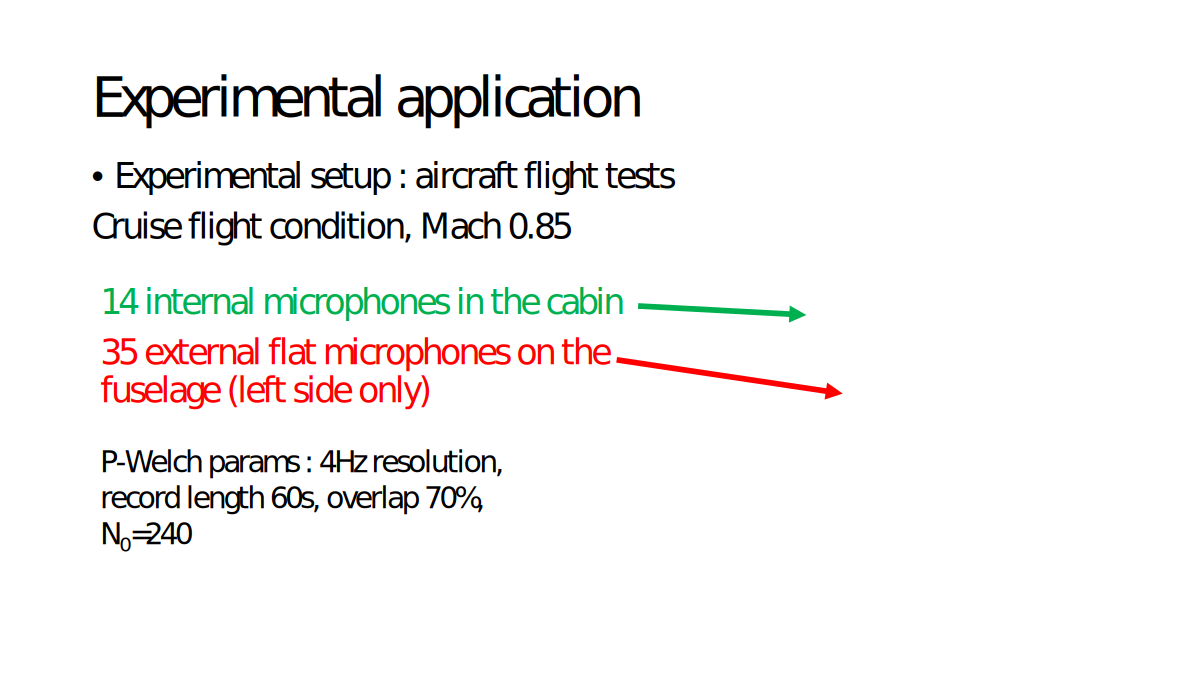
\includegraphics[width=\textwidth]{airbus/setup.png}};
		%\node[yshift=2.1cm,xshift=1.5cm,right,align=right] (b) at (current page) {{\scriptsize \textcolor{gray}{from Helffer, ICSV 2018}}\\ \includegraphics[width=0.4\textwidth]{airbus/setup2.png}};
		%\node at ($(current page)+(-2cm,-0.85cm)$) {\parbox{8cm}{

		\begin{itemize}
	        		\item Cruise flight condition: Mach 0.85\\	[1ex] 
	        		\item High engine speed + 1 background meas. (idle speed)\\	[1ex] 
	        		\item 33 microphones flushmounted on the aft  \tikzmark{ext} fuselage\\[1ex] 
	        		\item 9 microphones + 6 accelerometers in the cabin for reference only\tikzmark{int}		\\[1ex] 
	        		\item CSM:
	        		\begin{itemize}
	       		 	\item 4 Hz resolution
	       		 	\item 60 sec record length
	       		 	\item Hanning window
	       		 	\item overlap : 70\% (500 snapshots)
			\end{itemize}
			~\\		
%			\item Type of noise :
%			\begin{itemize}
%        				\item outside: TBL
%        				\item inside: air conditioning
%			\end{itemize}
		\end{itemize}
		\centering
		\vspace{-2cm}
		\hspace{-0.5cm}\includegraphics[width=0.55\textwidth]{/airbus/mic_pos_white.png} \hfill
		\includegraphics[width=0.44\textwidth]{airbus/setup2.png}\\
		 \footnotesize \textit{Outer microphone antenna}
		%\vspace{1.5cm}
		%}};
		%\draw[->,>=stealth,rouge,line width=1pt] ($(ext)+(0,1.7ex)$) [out=0,in=110]  to ($(a)+(3.2cm,1.5cm)$);%[out=0,in=110] 
		%\draw[->,>=stealth,source,line width=1pt] ($(int)+(0,1.7ex)$)  to ($(a)+(1.3cm,1.2cm)$);% [out=-45,in=135]
	%\end{tikzpicture}
\end{frame}

\captionsetup[subfigure]{labelformat=empty}
\begin{frame}{\insertsectionhead}
\small Autospectra of the outer mic. in the MF frequency range\\[-2em]

\parbox{\textwidth}{
	\begin{figure}
		{\centering
		\subfloat[\scriptsize \itshape Raw (high engine speed)]{\includegraphics[trim = 2ex 1ex 0 0,clip, width=0.32\textwidth]{./airbus/as_raw.png}}%Raw (high engine speed)
		\subfloat[\scriptsize \itshape Background noise (idle)]{\includegraphics[trim = 2ex 1ex 0 0,clip,width=0.32\textwidth]{./airbus/as_bg.png}} %Background noise (idle engine speed)
		\subfloat[\scriptsize \itshape After background subtraction ]{\includegraphics[trim = 1.2ex 1ex 0ex 0,clip,width=0.385\textwidth]{./airbus/as_bgsub.png}}}\\%Background subtraction
		\hfill \subfloat[\scriptsize  \itshape PFA denoising ]{\includegraphics[trim = 2ex 1ex 0 0,clip,width=0.32\textwidth]{./airbus/as_pfa.png}}%PFA denoising
		\subfloat[\scriptsize \itshape Reference-based denoising]{\includegraphics[trim = 2ex 1ex 0 0,clip,width=0.32\textwidth]{./airbus/as_ref.png}\hspace{-0.5cm}}\\% Referenced denoising
	\end{figure}
	}
	\begin{tikzpicture}[remember picture, overlay]
		\node[anchor=south west] (text) at ($(current page.south west)+(0.8cm,0.5cm)$) {
		\begin{minipage}[c][0.3\textwidth][l]{0.4\textwidth}
			\small
			\hspace{-0.3cm}\includegraphics[width=1.1\textwidth]{/airbus/mic_pos_white.png} 
			\vspace{0.5cm}
			%\includegraphics[height=0.5\textwidth]{airbus/jet.png}\\
			\uncover<2->{				
					%$\blacktriangleright$ BG subtraction gives\\ negative autospectra\\[0.8ex]
					 $\blacktriangleright$ Interference patterns:\tikzmark{bbsan} \\
					Regularly spaced monopoles in the jet (BBSAN)
%					\begin{center} 
%					\includegraphics[width=0.7\linewidth]{bbsan.png}\\
%					{\scriptsize \textcolor{gray}{From B. André, Ph.D. thesis, 2013}}
%					\end{center}
			}
			
		\end{minipage}
		};
		\uncover<2->{
			\node[draw, ellipse,minimum height=2.3cm, minimum width=1.3cm,anchor=west] (interf) at ($(current page.south west)+(6.2,2.8)$) {};
			%\draw[anchor=west] (interf) ellipse (2cm and 1cm);
			\draw[->,>=stealth,line width=1pt] ($(bbsan)+(0,2ex)$) to (interf); 
		}
	\end{tikzpicture}
\end{frame}


\begin{frame}{\insertsectionhead}	
	\small Autospectra averaged over the microphones
	\vfill
	\centering
	\includegraphics[width=0.7\textwidth]{airbus/mean_as_0-5.png}\\
	\vfill
	\small
		\begin{itemize}
        		\item Reduces the noise of 10-15 dB
        		\item PFA : Few denoising at very low frequency $\rightarrow$ TBL noise is correlated
       		 	%\item No extracted signal at high frequency  $\rightarrow$ inappropriate model
		\item PFA and reference-based denoising are in good agreement in the MF range
		
	\end{itemize}
\end{frame}

        
%\begin{frame}[t]{\insertsectionhead~--~Imaging}
%\centering
%\vspace{-0.2cm}
%\textbf{\footnotesize Inverse method}\\
%{\footnotesize Iterative Reweighted Least Squares, $p=0$ \\ and Bayesian regularization {\citeTransp{Antoni2019}}}\\[0.5ex]
%
%\begin{minipage}{1.1\textwidth} 	
% 		\hspace{-0.65cm}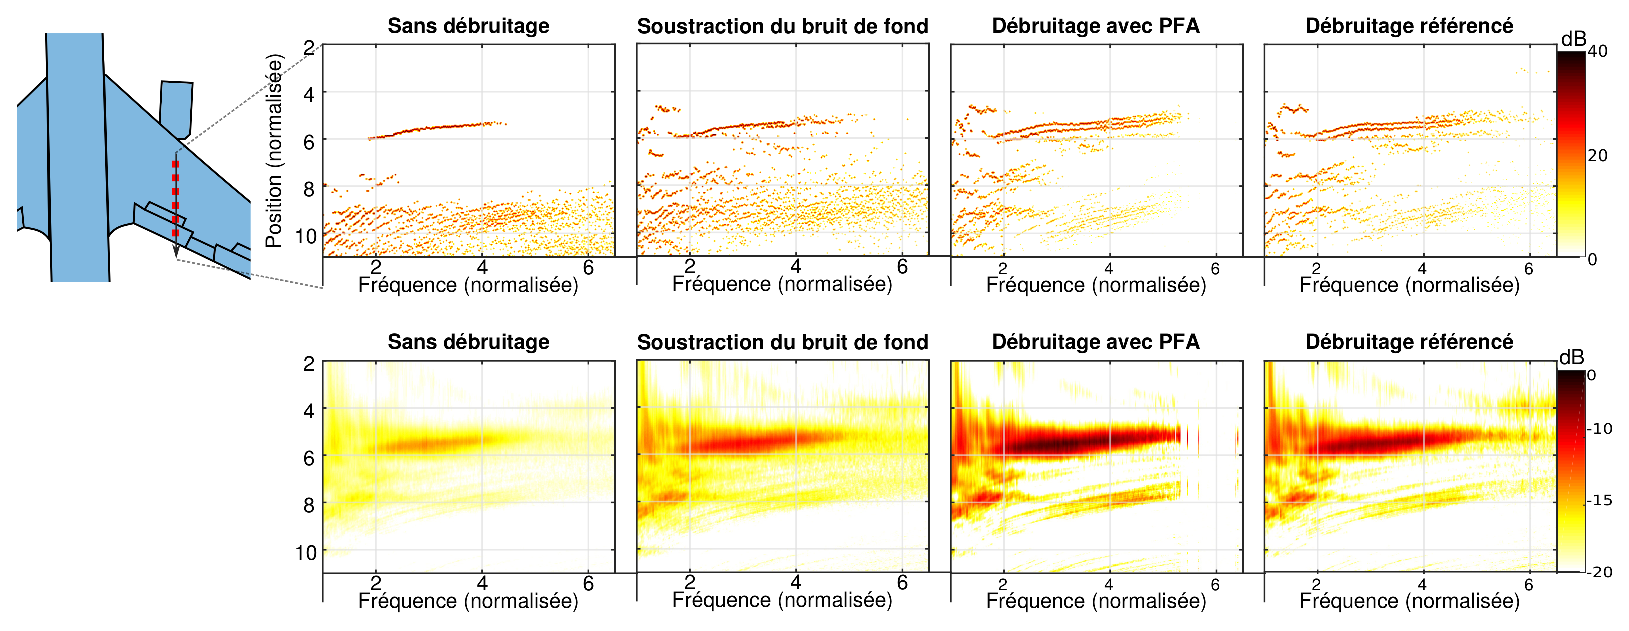
\includegraphics[width=\textwidth]{airbus/imagerie_final.eps}
% 		\begin{tikzpicture}[remember picture,overlay]
%     			\uncover<3->{\node[draw, ellipse,minimum height=1.8cm, minimum width=0.6cm,anchor=west]  at ($(current page.east)+(-3.2cm,1.55cm)$) {};}
%        	\end{tikzpicture}
% \end{minipage}~\\[0.5ex]
%\textbf{\footnotesize Coherence Beamforming}
%
%\vfill
%\onslide<2->{\small
%\flushleft
%	$\blacktriangleright$ Advanced denoising increase the dynamic of the beamforming map\\[0.5ex]
%        $\blacktriangleright$ 2 dominant wide-band sources $\rightarrow$ visible with advanced denoising\\[0.5ex]
%        \onslide<3->{$\blacktriangleright$ 4 correlated sources in the 1-2 frequency band (caused interference patterns)}
%        
%        
%}
%\end{frame}

%\begin{frame}[t]{\insertsectionhead~--~Imaging}
%{\footnotesize \bfseries Beamforming coherence}\\[2ex]
%\centering
%\begin{minipage}{1.1\textwidth} 	
% 		\hspace{-0.65cm}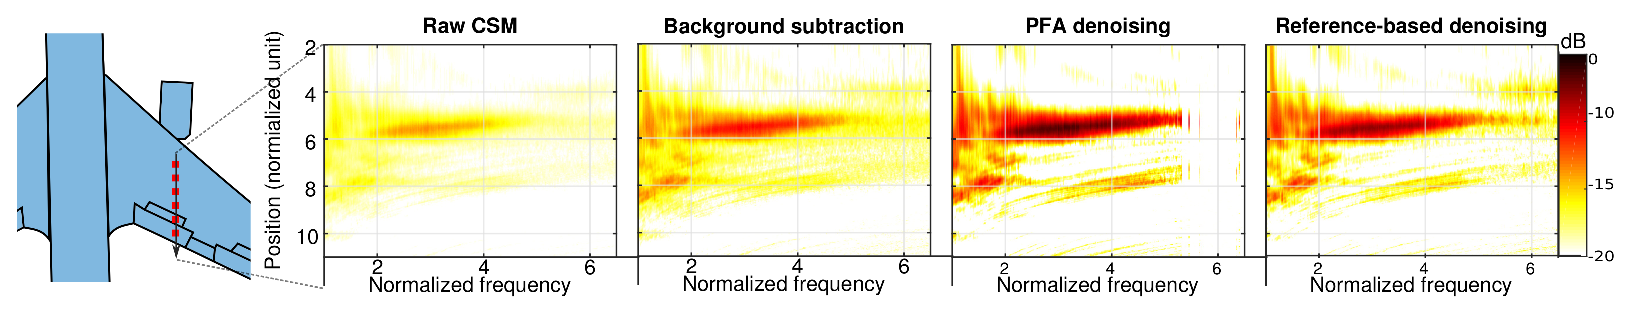
\includegraphics[width=\textwidth]{airbus/imagerie_beamforming.eps}
%
% \end{minipage}~\\[0.5ex]
%\vfill
%PFA : strong increase of the coherence
%
%\end{frame}

\begin{frame}[t]{\insertsectionhead~--~Imaging}

\textbf{\footnotesize Inverse method: }
{\footnotesize Iterative Reweighted Least Squares, $p=0$ \\\hspace{2cm} and Bayesian regularization {\scriptsize \citeTransp{Antoni2019}}}\\[2ex]
\centering
\begin{minipage}{1.1\textwidth} 	
 		\hspace{-0.65cm}\includegraphics[width=\textwidth]{airbus/imagerie_inverse.eps}
 		\begin{tikzpicture}[remember picture,overlay]
     			\uncover<3->{\node[draw, ellipse,minimum height=1.8cm, minimum width=0.6cm,anchor=west]  at ($(current page.east)+(-3.15cm,1.2cm)$) {};}
        	\end{tikzpicture}
 \end{minipage}~\\[0.5ex]
\vfill
\onslide<2->{\small
\flushleft
\begin{minipage}{0.6\textwidth}
        $\blacktriangleright$ 2 dominant wide-band sources\\ $\hookrightarrow$ visible only with advanced denoising\\[1ex]       
        \onslide<3->{$\! \blacktriangleright$ 4 correlated sources in the 1-2 frequency range\\$\hookrightarrow$ caused interference patterns} \\[1ex]       
        \onslide<4->{$\! \blacktriangleright$ PFA gives the lowest error        
        $$\displaystyle \scriptsize        \text{Error} = \frac{\|\bm{S}_{pp}^{\text{denoised}}-\bm{G}\bm{S}_{qq}\bm{G}'\|_1}{\|\bm{S}_{pp}^{\text{denoised}}\|_1+\|\bm{GS}_{qq}\bm{G}'\|_1}$$
        }
\end{minipage}
\hfill
\begin{minipage}{0.39\textwidth}
	\onslide<4->{\hfill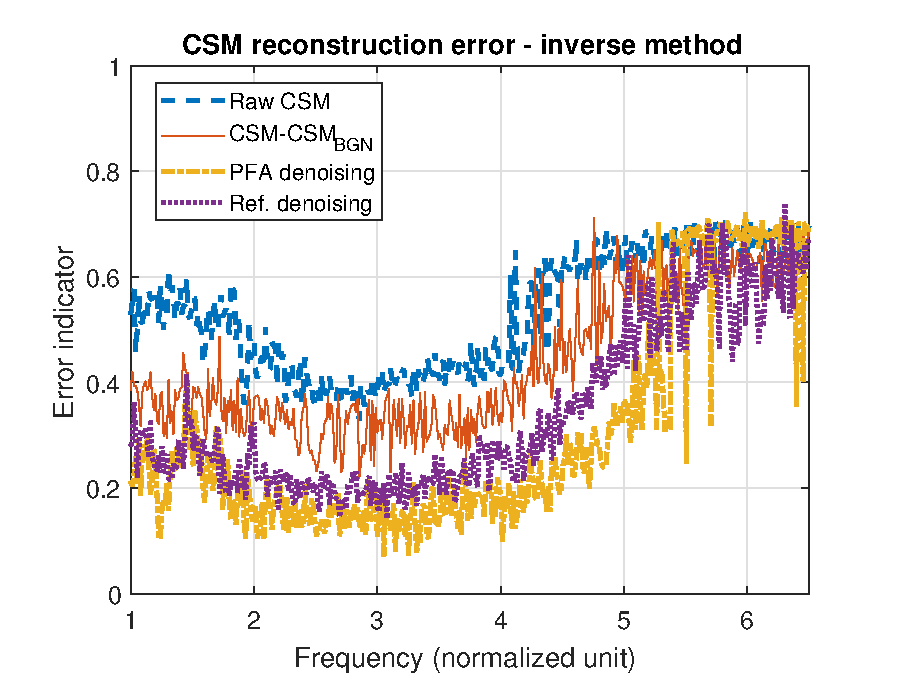
\includegraphics[width=0.9\textwidth]{airbus/errident.eps}\hspace{-0.5cm}}

\end{minipage}
	 
}
\end{frame}

%\begin{frame}{\insertsectionhead~--~Imaging}
%	\centering
%	\small
%	\begin{equation*}
%        		\text{Error} = \frac{\|\bm{S}_{pp}^{\text{denoised}}-\bm{G}\bm{S}_{qq}\bm{G}'\|_1}{\|\bm{S}_{pp}^{\text{denoised}}\|_1+\|\bm{GS}_{qq}\bm{G}'\|_1}
%	\end{equation*}
%	\begin{itemize}
%        		\item $\bm{G}$ Convected Green’s functions between sources and microphones
%        		\item From the beamforming map (left): based only on the maximum location
%\end{itemize}
%	\vfill
%	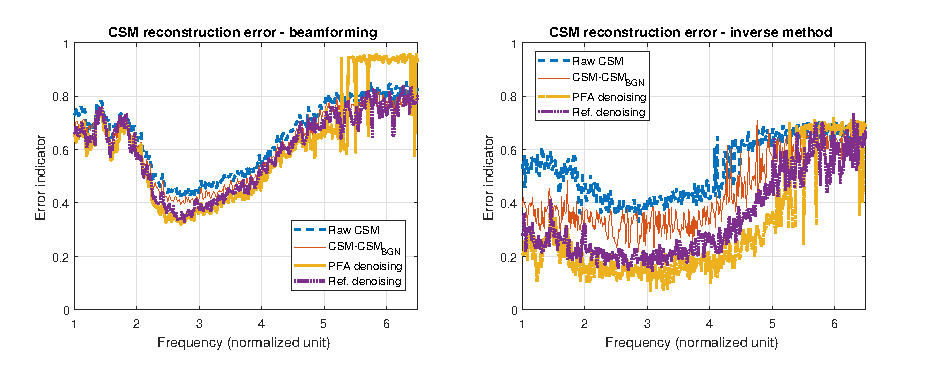
\includegraphics[width=0.9\textwidth]{airbus/erreur.eps}
%\end{frame}

\begin{frame}{Conclusions}
	\vspace{2.5em}
\begin{itemize}
	\item Denoising with different requirements/hypothesis\\
%	\hspace{-0.8cm}\begin{minipage}[t]{0.43\textwidth}
%		\begin{block}{Reference denoising: }
%			\begin{itemize}
%       				 \item Noise-free reference channels
%       			 	 \item Rely on one measurement\\~
%			\end{itemize}
%		\end{block}
%	\end{minipage}
%	\hfill
%	\begin{minipage}[t]{0.55\textwidth}
%		\begin{block}{PFA denoising:}
%			\begin{itemize}
%				\item No reference channel
%	       			 \item Extract a common noise from several measurements including background 
%			\end{itemize}
%		\end{block}
%	\end{minipage}\\
%	~\\[1ex]	
	$\hookrightarrow$ but both give similar results\\
	\vspace{2.5em}
        \item Denoising increases of the imaging performance
	\vspace{2.5em}
	\item Possible improvements for PFA:
	\begin{itemize}
        		\item use a more efficient/robust solver
        		\item change the model to have better control on sparsity level% adapter le modèle statistique (meilleur contrôle de la parcimonie)
        		\item account for a correlated noise model for the low-frequency range% prendre en compte la corrélation du bruit en BF
	\end{itemize}
\end{itemize}

\vspace{1cm}

\begin{center}
	\noindent\rule{\textwidth}{0.4pt}
	\textcolor{black!70}{\scriptsize \itshape{ 
	\centering This work was performed in the framework of Clean Sky 2 Joint Undertaking, European Union (EU), Horizon 2020, CS2-RIA, ADAPT project, Grant agreement no 754881.}}
\end{center}
\end{frame}



\appendix
\begin{frame}{References}
	%\begin{adjustwidth}{-2em}{-2.5em}
		\setlength{\bibsep}{2em}
		\bibliographystyle{abbrvnat}
		\bibliography{biblio}
	%\end{adjustwidth}
\end{frame}
%%% APPENDIX
\newcounter{finalframe}
\setcounter{finalframe}{\value{framenumber}}

\begin{frame}{Appendix -- Beamforming}
	\centering
	\footnotesize Iterative Reweighted Least Squares, $p=0$ \\ and Bayesian regularization\\~\\
	\begin{minipage}{1.1\textwidth}
			\hspace{-0.65cm}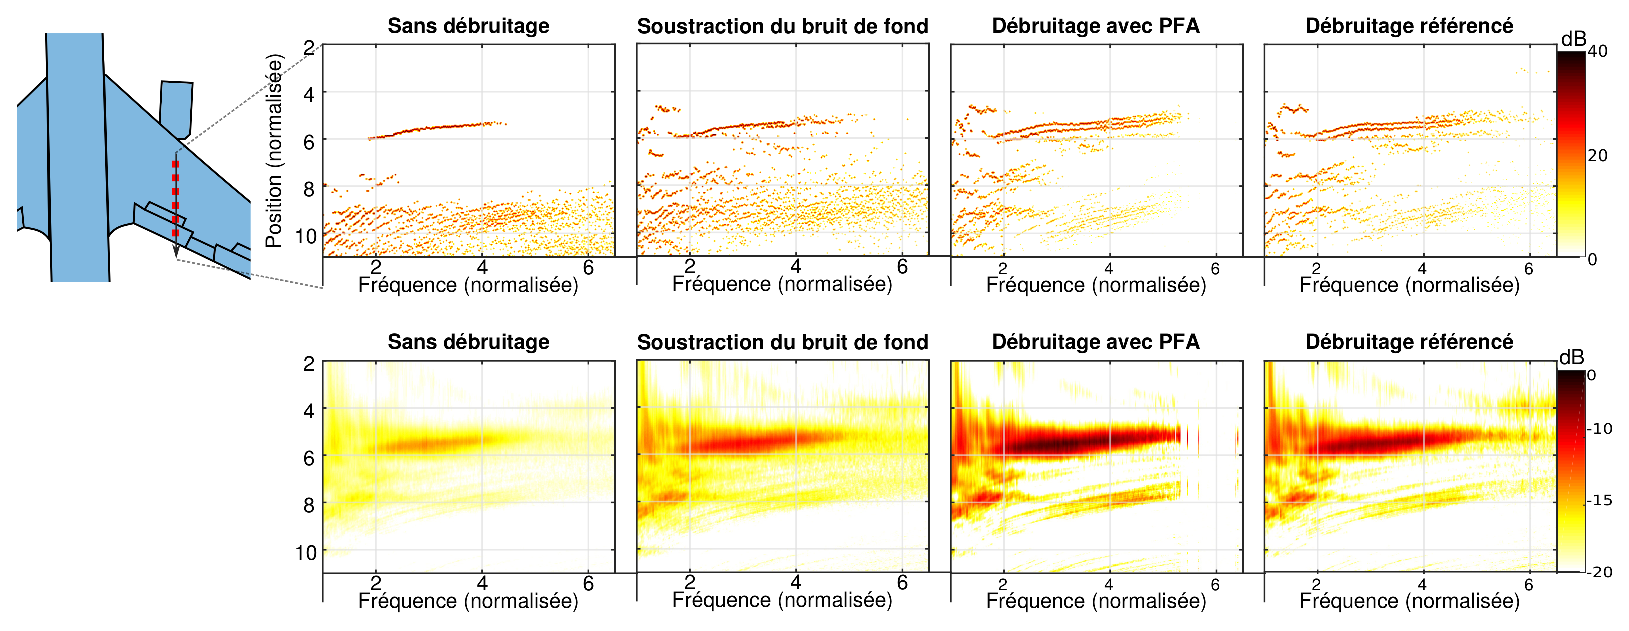
\includegraphics[width=1\textwidth]{airbus/imagerie_final.eps}\\
\end{minipage}

	Beamforming coherence

\end{frame}

\begin{frame}{Appendix -- Credible interval}
\centering
\includegraphics[width=0.8\textwidth]{ic_95pc.png}\\
In gray : 95\% credible interval for PFA denoising
\end{frame}
\setcounter{framenumber}{\value{finalframe}}

\end{document}